\chapter{Chuỗi Markov là gì ?}

\section{Mở đầu}
\begin{defivn}
    Một \textbf{quá trình ngẫu nhiên} là một chuỗi biến ngẫu nhiên $(X_t)_{t \geq 0}$ trên một không gian mẫu $\Omega$, được đánh số bởi thời gian $t$ và các biến ngẫu nhiên có giá trị nằm trong một tập hợp $S$, gọi là \textbf{không gian trạng thái}.
\end{defivn}
\vspace{5pt}

\begin{egvn}
    Xét $X_n$ là vị trí của một con cua tại thời điểm $t = n$ (di chuyển ngang, xem như di chuyển trên trục $x$). Con cua có xác suất $0.67$ để di chuyển sang trái, có xác suất $0.33$ để di chuyển sang phải, tại thời điểm đầu tiên, con cua đứng yên nên $X_0 = 0$, tại thời điểm tiếp theo, con cua sẽ di chuyển sang trái nên $X_1 = -1$, nhưng thời điểm tiếp theo nữa, con cua lại di chuyển sang phải nên $X_2 = 0$, và cứ ngẫu nhiên như thế.
\end{egvn}

\begin{itemize}
    \item Trong phạm vi này, ta chỉ xét quá trình ngẫu nhiên \textbf{thời gian rời rạc}, nghĩa là $t$ có giá trị từ $0, 1, 2, ...$ hay nói cách khác, $t \in E$ với $E \subseteq \N$.
    
    \item Để một quá trình ngẫu nhiên trở thành một chuỗi Markov (ta chỉ xét chuỗi Markov thời gian rời rạc), ta cần thoả 3 điều kiện dưới đây:
    \begin{itemize}
        \item Là quá trình ngẫu nhiên thời gian rời rạc.
        \item Không gian trạng thái $S$ là một tập hợp đếm được (ta sẽ tập trung xét $S$ là hữu hạn) và $X_i$ là biến ngẫu nhiên rời rạc.
        \item Có \textbf{tính chất Markov}.
    \end{itemize}

    \item Ta có thể hiểu tính chất Markov đơn giản như sau "Xác suất của trạng thái tiếp theo của quá trình ngẫu nhiên chỉ phụ thuộc vào hiện tại mà không phụ thuộc vào quá khứ".
\end{itemize}

%%%%%%%
\section{Định nghĩa}

\begin{defivn} Một quá trình ngẫu nhiên thoả mãn \textbf{Tính chất Markov} nếu:
$$
\P(X_{n + 1} = s \mid X_0 = x_0, X_1 = x_1, ..., X_n = x_n) = \P(X_{n+1} = s \mid X_n = x_n)
$$
với mọi $n \geq 0$ và với mọi $s, x_0, x_1, ..., x_n \in S$. Và ta gọi quá trình ngẫu nhiên trên là một \textbf{Chuỗi Markov}.
\end{defivn}

\begin{defivn}
    Một chuỗi Markov được nói là \textbf{đồng nhất} nếu:
    $$
    \P(X_{n+1} = y \mid X_{n} = x) = \P(X_1 = y \mid X_0 = x)
    $$
    với mọi $x, y \in S$ và với mọi $n \geq 0$.
\end{defivn}

\begin{itemize}
    \item Từ đây trở về sau, ta sẽ chỉ dùng đến chuỗi Markov đồng nhất.
    
    \item Ngoài ra ta sẽ kí hiệu $P_{xy}$ cho xác suất có điều kiện $P(X_1 = y \mid X_0 = x)$ $\forall x,y \in S$ và gọi là \textbf{xác suất chuyển tiếp 1-bước}.
    
    \item Và cuối cùng điều quan trọng nhất đối với một chuỗi Markov có không gian trạng thái hữu hạn hay $S = \{x_0, x_1, ..., x_n \}$, đó là \textbf{phân phối ban đầu}, đặt là $\pi_0$ và đặt $\pi_{0}(x_i) = \P(X_0 = x_i)$ với $x_i \in S$. Lúc này ta có:
    $$
    \pi_0 = \begin{bmatrix}
        \pi_{0}(x_0) & \pi_{0}(x_1) & ... \pi_{0}(x_n) \\
    \end{bmatrix}
    $$

    \item Tương tự với mỗi biến ngẫu nhiên $X_i$ ta sẽ kí hiệu $\pi_i$ là phân phối của nó.

    \item Do $S = \{x_0, x_1, ..., x_n \}$ là một tập hợp hữu hạn nên thông thường ta đưa về dạng ma trận gồm các xác suất chuyển tiếp 1-bước mà chuỗi Markov có thể có, kí hiệu là $\mathbf{P}$ và gọi ma trận đó là \textbf{ma trận chuyển tiếp} hay \textbf{ma trận Markov}, ta có:
    $$
    \mathbf{P} = \begin{bmatrix}
        P_{x_0x_0} & P_{x_0x_1} & ... & P_{x_0x_n} \\
        P_{x_1x_0} & P_{x_1x_1} & ... & P_{x_1x_n} \\
        \vdots & \vdots & \ddots & \vdots \\
        P_{x_nx_0} & P_{x_nx_1} & ... & P_{x_nx_n} \\
    \end{bmatrix}
    $$
\end{itemize}

\begin{defivn}
    Một ma trận vuông được gọi là \textbf{ma trận ngẫu nhiên} nếu thoả mãn 2 điều kiện sau:
    \begin{itemize}
        \item[(a)] Tổng các phần tử của mỗi dòng đều là 1.
        \item[(b)] Mọi phần tử đều không âm.
    \end{itemize}

\noindent Ta có thể thấy ma trận chuyển tiếp $\mathbf{P}$ luôn luôn là một ma trận ngẫu nhiên.
\end{defivn}

% \begin{defivn}
%     Cho $(X_n)_{n \geq 0}$ là một chuỗi Markov trên không gian trạng thái $S$ (ta gọi một phần tử $x \in S$ là một trạng thái) khi đó một trạng thái $x \in S$ được gọi là \textbf{trạng thái hấp thụ} nếu $P_{xx} = 1$.
% \end{defivn}

\begin{theovn}
    Cho một chuỗi Markov $(X_n)_{n \geq 0}$ với một không gian trạng thái $S$ hữu hạn. Đặt thời gian $i$ là thời điểm hiện tại, khi đó thời điểm quá khứ và tương lai của chuỗi Markov độc lập lẫn nhau. Nghĩa là, với mọi $n > i$ và với mọi $x_0, x_1, ..., x_{i-1}, x_i, x_{i+1}, ..., x_n \in S$, ta có:
    $$
    \begin{aligned}
    &\P(X_0 = x_0, ..., X_{i-1} = x_{i-1}, X_{i+1} = x_{i+1}, ..., X_n = x_n \mid X_i = x_i) \\
    = &\P(X_0 = x_0, ..., x_{i-1} = x_{i-1} \mid X_i = x_i) \P(X_{i+1} = x_{i+1}, ..., X_n = x_n \mid X_i = x_i)
    \end{aligned}
    $$
\end{theovn}
\begin{proofvn} \vphantom{}
    \begin{itemize}
        \item Đặt $F = (X_0 = x_0, ..., X_{i-1} = x_{i - 1})$, $E = (X_{i+1} = x_{i+1}, ..., X_n = x_n)$ và $G = (X_i = x_i)$, ta có:
        $$
        \begin{aligned}
            \P(E \cap F \mid G) &= \dfrac{\P(E \cap F \cap G)}{\P(G)} \\
            &= \dfrac{\P(E \cap F \cap G)}{\P(F \cap G)} \dfrac{\P(F \cap G)}{\P(G)} \\
            &= \P(E \mid F \cap G)\P(F \mid G) \\
            &= \P(E \mid G)\P(F \mid G) \hspace{10pt} \text{(áp dụng tính chất của chuỗi Markov)}
        \end{aligned}
        $$

        \item Vậy:
        $$
        \begin{aligned}
        &\P(X_0 = x_0, ..., X_{i-1} = x_{i-1}, X_{i+1} = x_{i+1}, ..., X_n = x_n \mid X_i = x_i) \\
        = &\P(X_0 = x_0, ..., x_{i-1} = x_{i-1} \mid X_i = x_i) \P(X_{i+1} = x_{i+1}, ..., X_n = x_n \mid X_i = x_i)
        \end{aligned}
        $$
    \end{itemize}
\end{proofvn}

\begin{itemize}
    \item Ngoài ra để có thể hình dung tốt hơn Chuỗi Markov, ta có thể biểu diễn nó thành một đồ thị.

    \item Xét ví dụ một chuỗi Markov chỉ có 2 trạng thái, hay nói cách khác $S$ chỉ có 2 phần tử. Xét $S = \{0, 1\}$, ta có $P_{01} = a$ và $P_{10} = b$. Khi đó ma trận chuyển tiếp $\mathbf{P}$ sẽ là:
    $$
    \mathbf{P} = \begin{bmatrix}
        P_{00} & P_{01} \\
        P_{10} & P_{11} \\
    \end{bmatrix} = \begin{bmatrix}
        1 - a &  a \\
        b & 1 - b
    \end{bmatrix}
    $$

    \item Đồ thị biểu diễn cho chuỗi Markov là một đồ thị $G = (V, E)$ (với $V = S$) \textit{có hướng} và \textit{có trọng số} với các trọng số chính là các xác suất chuyển tiếp từ trạng thái này sang trạng thái khác hay từ đỉnh này sang đỉnh khác.
\end{itemize}

\begin{figure}[H]
    \centering
    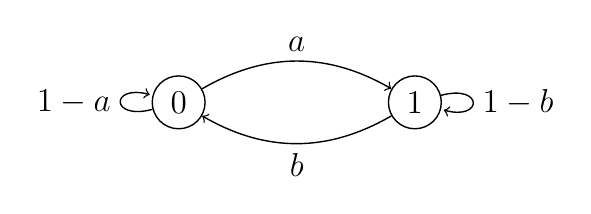
\begin{tikzpicture}[-> , line width=0.5 pt ,node distance =2 cm]
        \tikzstyle{every node}=[font=\large]
        \node[circle, draw] (zero) at (0,0) {0};
        \node[circle, draw] (one) at (3,0) {1};
        \path (zero) edge [bend left] node [above] {$a$} (one);
        \path (zero) edge [loop left] node{$1-a$} (zero);
        \path (one) edge [bend left] node [below] {$b$} (zero);
        \path (one) edge [loop right] node{$1-b$} (one);
    \end{tikzpicture}
    \caption{Đồ thị $G$ biểu diễn của chuỗi Markov 2 trạng thái}
    \label{fig:22graph}
\end{figure}
